\section{Confronto}
Sicuramente l'algoritmo con costo computazionale più basso è Kruskal con Union-Find.
Confrontiamo quindi l'esecuzione di Kruskal con Union-Find con gli altri due algoritmi partendo da Prim. 
\begin{figure}[H]
\centering
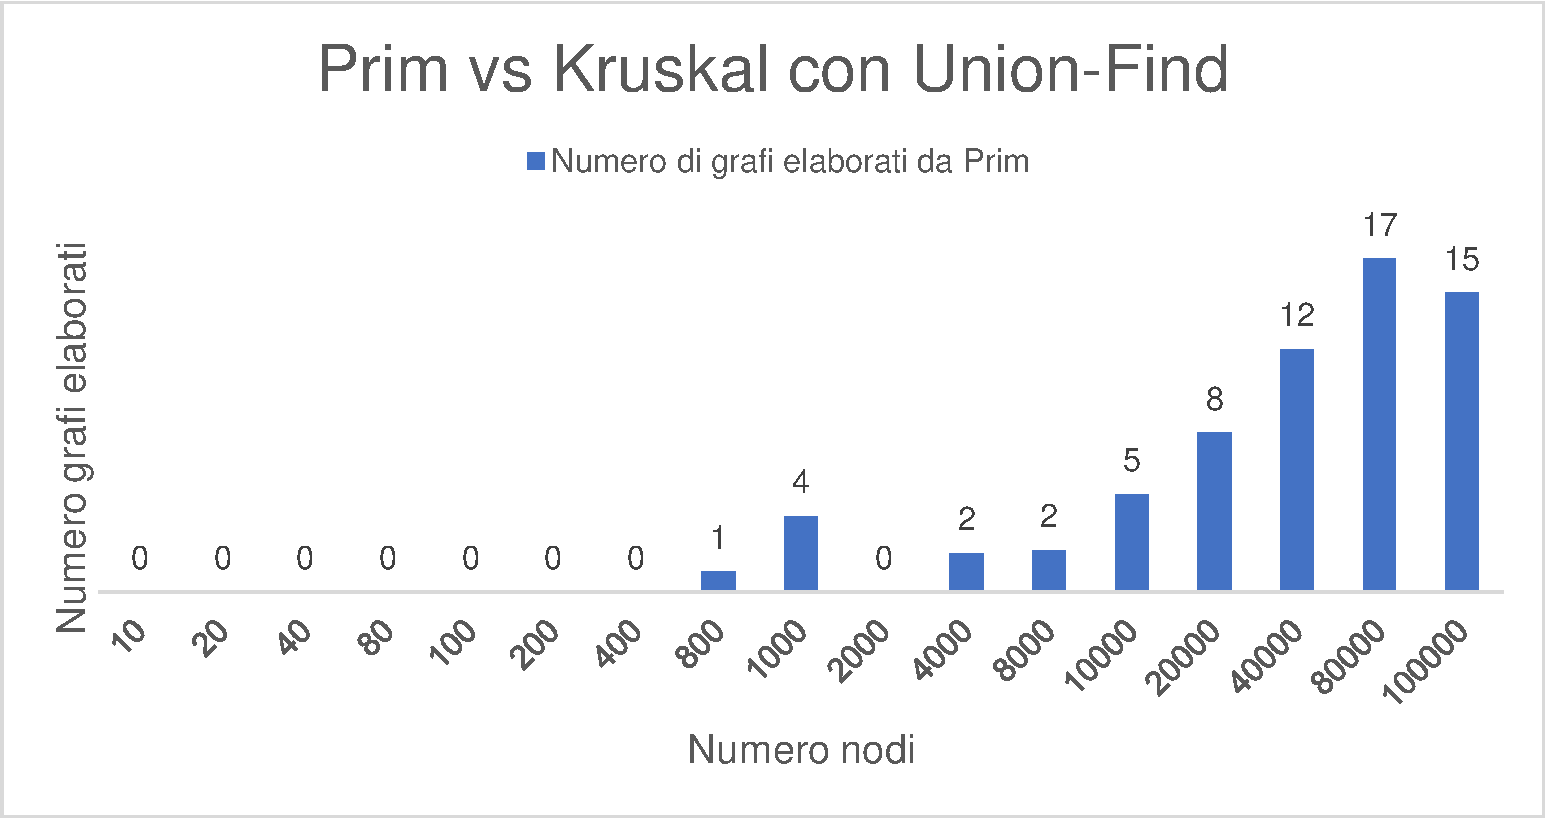
\includegraphics[scale=0.5]{grafici/primvskruskaluf.pdf}
\caption{Numero di grafi di dimensione $n$ che Kruskal con Union-Find è in grado di elaborare nello stesso tempo medio impiegato da Prim per elaborare \textbf{un} grafo  della medesima dimensione. Come possiamo vedere Kruskal è molto più efficiente in grafi di grandi dimensioni.}
\end{figure}
Confrontiamo ora l'algoritmo di Kruskal con Union-Find con la sua versione naive:
\begin{figure}[H]
\centering
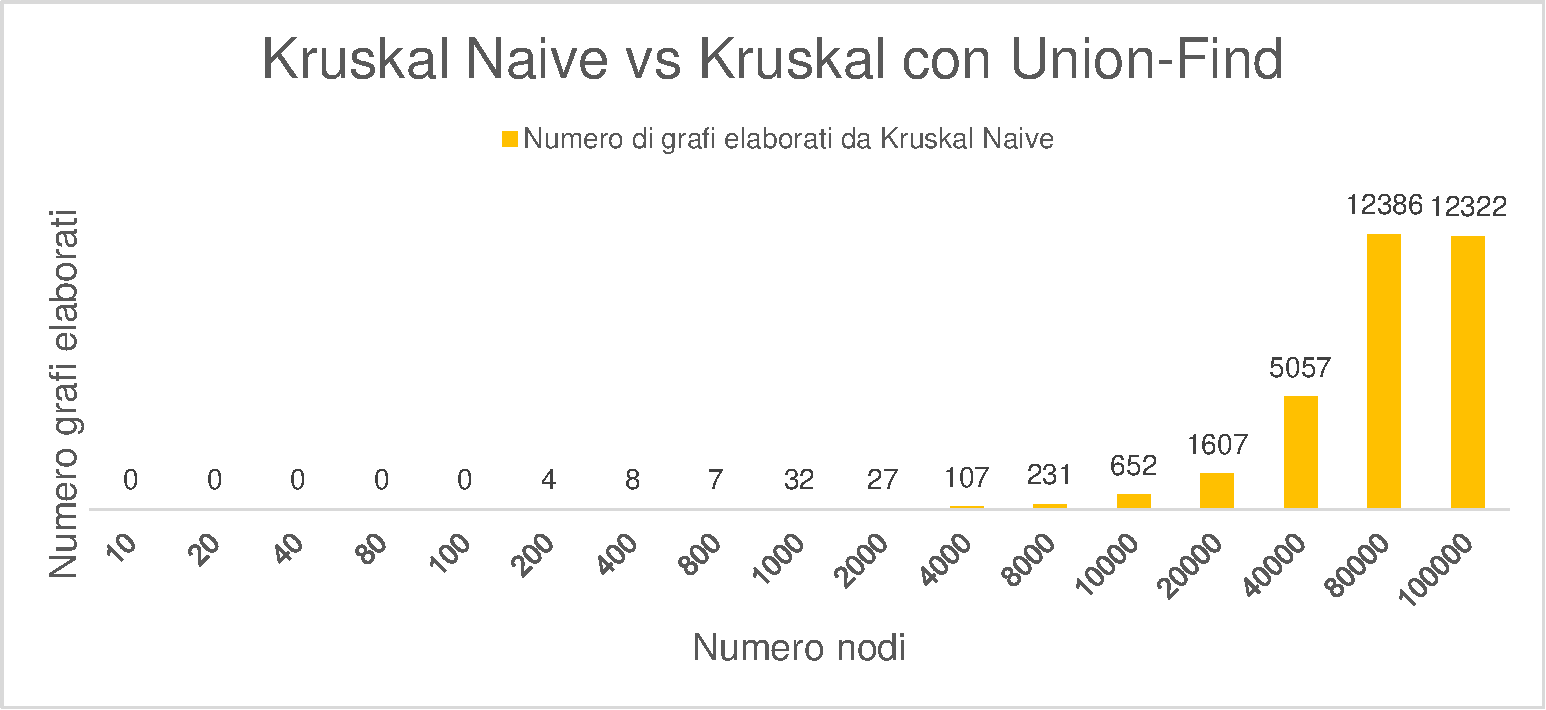
\includegraphics[scale=0.5]{grafici/kruskalvskruskaluf.pdf}
\caption{Numero di grafi di dimensione $n$ che Kruskal con Union-Find è in grado di elaborare nello stesso tempo medio impiegato da Kruskal per elaborare \textbf{un} grafo della medesima dimensione. Come possiamo vedere Kruskal è molto più efficiente in grafi di grandi dimensioni.}
\end{figure}
Da questi due grafici e nella tabella \ref{t1} possiamo affermare che Kruskal con Union-Find è l'algoritmo \textbf{più} efficiente per il calcolo di un MST, segue l'algoritmo di Prim, e infine Kruskal "Naive" che ha il costo computazionale più alto.
\section{Conclusione}
I risultati ottenuti rispecchiano l'andamento che ci aspettavamo conoscendo la complessità degli algoritmi, infatti Kruskal "Naive" di complessità $O(mn)$ ha ottenuto risultati peggiori di qualche ordine di grandezza rispetto agli altri due algoritmi, i quali hanno entrambi complessità $O(m\log{}n)$.

La differenza tra Kruskal con Union-Find e Prim è dovuta probabilmente dalla nostra implementazione degli algoritmi e delle strutture dati che abbiamo utilizzato, ad esempio esistono implementazioni migliori di Prim che utilizzano Heap di Fibonacci per abbassare la complessità a $O(m+n\log{}n)$ e che avrebbero portato a tempi di esecuzione più bassi per i grafi di dimensione maggiore.

In termini di efficienza Kruskal con Union-Find ha ottenuto i tempi di esecuzione più bassi sia per grafi di piccola dimensione sia per i grafi con più di 80000 nodi, ed è quindi l'algoritmo migliore nella nostra implementazione. 